\documentclass{standalone}
\usepackage{tikz}
\usetikzlibrary{positioning}
\usetikzlibrary{calc}

\begin{document}

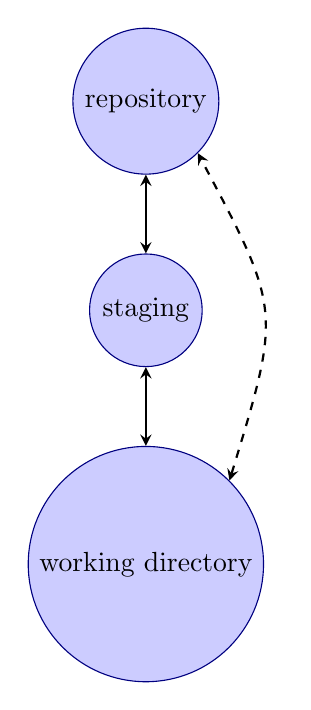
\begin{tikzpicture}[
workingdir/.style={circle,
                fill=blue!20!white,
                draw=blue!50!black,
                minimum size=5mm},
staging/.style={circle,
                fill=blue!20!white,
                draw=blue!50!black,
                minimum size=5mm},
repo/.style={circle,
                fill=blue!20!white,
                draw=blue!50!black,
                minimum size=5mm},
link/.style={-, >=stealth, thick}]

% box to represent .git dir
% git add, git commit text
% git commit <file>; git commit -a


\node (working dir) at (0, 0) [workingdir] {working directory};
\node (staging) [staging, above=of working dir] {staging};
\draw [link, <->] (working dir) -- (staging);
\node (repo) [repo, above=of staging] {repository};
\draw [link, <->] (staging) -- (repo);

\draw [link, <->, dashed] (working dir.north east)
    .. controls ($ (staging.east) + (1, 0) $) .. (repo.south east);

\end{tikzpicture}
\end{document}
